\documentclass[10pt,a4paper]{article}
\usepackage[top=1.4cm, bottom=1.4cm, left=1.6cm, right=1.6cm, headheight=14pt, footskip=18pt]{geometry}
\usepackage[utf8]{inputenc}
\usepackage{amsmath,amsfonts,amssymb}
\usepackage{graphicx}
\usepackage{tikz}
\usepackage{circuitikz}
\usetikzlibrary{calc,patterns}
\usepackage[most]{tcolorbox}
\usepackage{enumitem}
\usepackage{fancyhdr}
\usepackage{booktabs}
\usepackage{tabularx}
\usepackage{colortbl}
\usepackage{hyperref}

% --- Palet Warna Resmi UNIB ---
\definecolor{unibblue}{RGB}{0, 32, 96}
\definecolor{unibgold}{RGB}{197, 160, 89}
\definecolor{unibgreen}{RGB}{34, 112, 60}
\definecolor{boxbg}{RGB}{248, 250, 253}
\definecolor{linegray}{RGB}{210, 215, 225}

% --- Pengaturan Header & Footer ---
\pagestyle{fancy}
\fancyhf{}
\lhead{\footnotesize\textbf{\color{unibblue}Universitas Bengkulu} \textbar\ Program Studi S1 Teknik Elektro}
\rhead{\footnotesize\color{gray}Persamaan Diferensial (Genap 2026)}
\lfoot{\footnotesize\color{gray}Problem Set OBE \textbar\ \textbf{Video}: \url{https://youtu.be/oEBvpt86fvI} \textbar\ \href{https://www.youtube.com/playlist?list=PLS5oOZWXZeTw}{\color{unibblue}\textbf{Playlist}}}
\cfoot{\footnotesize\color{gray}Hal. \thepage\ dari 2}
\rfoot{\footnotesize\color{unibblue}\textbf{Minggu 10: Deret Fourier Eksponensial \& Kek...}}
\renewcommand{\headrulewidth}{0.6pt}
\renewcommand{\footrulewidth}{0.4pt}

\begin{document}

% ==================== HALAMAN 1 ====================
\noindent\begin{minipage}[c]{0.68\textwidth}%
  {\large\textbf{\color{unibblue}PROBLEM SET (TUGAS MANDIRI TERSTRUKTUR)}}\\[1mm]
  {\normalsize\textbf{Mata Kuliah: Persamaan Diferensial (2 SKS)}}\\[0.5mm]
  {\small\textbf{Topik Minggu 10:} Deret Fourier Eksponensial \& Kekekalan Daya Parseval}%
\end{minipage}%
\hfill%
\begin{minipage}[c]{0.30\textwidth}%
  \begin{tcolorbox}[colback=unibblue!5,colframe=unibblue,boxrule=0.6pt,arc=2pt,left=4pt,right=4pt,top=2pt,bottom=2pt]
    \scriptsize
    \textbf{Nama:} \dotfill\\[1.2mm]
    \textbf{NPM:} \dotfill\\[1.2mm]
    \textbf{Kelas/Klp:} \dotfill\\[1.2mm]
    \textbf{Nilai Final:} \hfill \textbf{/ 100}
  \end{tcolorbox}%
\end{minipage}\par

\vspace{1.5mm}

% Kotak Sub-CPMK & Pedoman Tugas Terstruktur
\begin{tcolorbox}[colback=boxbg,colframe=unibgold!90!black,boxrule=0.6pt,arc=2pt,left=5pt,right=5pt,top=3pt,bottom=3pt,title=\textbf{\scriptsize Capaian Pembelajaran (Sub-CPMK 5) \& Pedoman Pengerjaan Tugas}]
  \scriptsize
  \textbf{Sub-CPMK 5:} Mahasiswa mampu mentransformasikan deret Fourier ke dalam bentuk eksponensial kompleks serta menerapkan Teorema Parseval untuk menganalisis disipasi daya pada beban harmonisa.\\
  \textbf{Video Perkuliahan (YouTube):} \url{https://youtu.be/oEBvpt86fvI} \hfill \textbf{Playlist:} \href{https://www.youtube.com/playlist?list=PLS5oOZWXZeTw}{\color{unibblue}\textbf{bit.ly/pd-unib-playlist}}\\\textbf{Ketentuan Tugas:} Kerjakan secara mandiri pada kertas folio/A4 bergaris atau laporan digital rapi. Lampirkan penurunan rumus analitis lengkap dan cetak visualisasi kode program Julia (Soal C6). Kumpulkan pada awal perkuliahan minggu berikutnya.
\end{tcolorbox}

\vspace{1.5mm}

\noindent{\textbf{\color{unibblue}\large BAGIAN I: FONDASI KONSEPTUAL \& PENURUNAN MATEMATIS}}\par
\vspace{1mm}

% Soal C1
\noindent\textbf{1. (C1 - Mengingat \textbar\ Bobot: 10 Poin)}\par\vspace{0.8mm}
{\footnotesize Tuliskan bentuk Deret Fourier eksponensial kompleks $f(t) = \sum_{n=-\infty}^{\infty} c_n e^{j n \omega_0 t}$ dan rumus integral untuk spektrum koefisien kompleks $c_n$. Bagaimana hubungan antara $c_n$ dengan koefisien trigonometrik $a_n$ dan $b_n$?}\par

\vspace{2.5mm}

% Soal C2
\noindent\textbf{2. (C2 - Memahami \textbar\ Bobot: 15 Poin)}\par\vspace{0.8mm}
{\footnotesize Jelaskan makna fisis Teorema Parseval dalam konteks kekekalan energi dan daya listrik: mengapa total daya aktif rata-rata yang diserap beban linier merupakan jumlahan skalar dari daya masing-masing harmonisa tanpa adanya interaksi silang antar-frekuensi berbeda?}\par

\vspace{2.5mm}

% Soal C3
\noindent\textbf{3. (C3 - Menerapkan \textbar\ Bobot: 20 Poin)}\par\vspace{0.8mm}
\noindent\begin{minipage}[t]{0.60\textwidth}%
  {\footnotesize Tinjau bentuk gelombang tegangan segitiga simetris bolak-balik pada gambar di samping dengan periode $T = 10\text{ ms}$ dan nilai puncak $V_p = 100\text{ V}$. Turunkan koefisien deret Fourier eksponensial $c_n$ secara tuntas untuk seluruh indeks bilangan bulat $n \in \mathbb{Z}$.}%
\end{minipage}%
\hfill%
\begin{minipage}[t]{0.37\textwidth}%
  \centering
  \resizebox{0.95\linewidth}{!}{%
  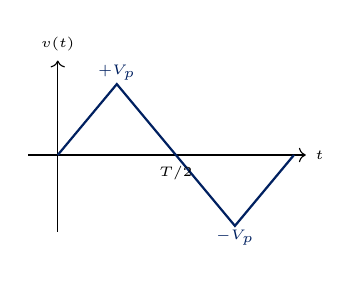
\begin{tikzpicture}[scale=0.75]
    \draw[->] (-0.5,0) -- (4.2,0) node[right, font=\tiny] {$t$};
    \draw[->] (0,-1.3) -- (0,1.6) node[above, font=\tiny] {$v(t)$};
    \draw[thick, unibblue] (0,0) -- (1.0,1.2) -- (2.0,0) -- (3.0,-1.2) -- (4.0,0);
    \node at (1.0,1.4) [font=\tiny\bfseries, unibblue] {$+V_p$};
    \node at (3.0,-1.4) [font=\tiny\bfseries, unibblue] {$-V_p$};
    \node at (2.0,-0.3) [font=\tiny] {$T/2$};
  \end{tikzpicture}%
  }%
\end{minipage}\par

\vfill

% Kotak Formula Rujukan Teknis & Standar Industri
\begin{tcolorbox}[colback=unibblue!3,colframe=unibblue,colbacktitle=unibblue,coltitle=white,boxrule=0.6pt,arc=2pt,left=6pt,right=6pt,top=3pt,bottom=3pt,title=\textbf{\scriptsize FORMULA RUJUKAN TEKNIS \& STANDAR INDUSTRI TERKAIT}]
  \scriptsize
  \begin{itemize}[leftmargin=*, nosep]
  \item Simetri Fungsi: Genap ($f(-t) = f(t) \implies b_n = 0$), Ganjil ($f(-t) = -f(t) \implies a_n = 0$)
  \item Teorema Parseval (Kekekalan Daya): $P_{\text{avg}} = I_{\text{rms}}^2 R = R \left[ I_0^2 + \sum_{n=1}^\infty \frac{I_{n,\text{maks}}^2}{2} \right]$
  \item Nilai Efektif (RMS) Sinyal Terdistorsi: $I_{\text{rms}} = \sqrt{I_{\text{dc}}^2 + I_{1,\text{rms}}^2 + I_{2,\text{rms}}^2 + \dots}$
  \item Faktor Daya Sejati (*True Power Factor*): $\text{PF}_{\text{true}} = \frac{P}{S} = \frac{I_{1,\text{rms}}}{I_{\text{rms}}} \cos\theta_1$
\end{itemize}
\end{tcolorbox}

\newpage
% ==================== HALAMAN 2 ====================

\noindent{\textbf{\color{unibblue}\large BAGIAN II: ANALISIS SISTEM, EVALUASI STANDAR, \& KOMPUTASI JULIA}}\par
\vspace{1mm}

% Soal C4
\noindent\textbf{4. (C4 - Menganalisis \textbar\ Bobot: 20 Poin)}\par\vspace{0.8mm}
{\footnotesize Tegangan segitiga dari Soal 3 dihubungkan ke sebuah elemen pemanas berhambatan murni $R = 10\,\Omega$. (a) Hitung daya aktif rata-rata fundamental $P_1$; (b) Gunakan Teorema Parseval untuk menghitung persentase kontribusi daya harmonisa ke-3 dan ke-5 terhadap disipasi kalor total; (c) Analisis rugi daya tambahan akibat keberadaan harmonisa.}\par

\vspace{3.5mm}

% Soal C5
\noindent\textbf{5. (C5 - Mengevaluasi \textbar\ Bobot: 20 Poin)}\par\vspace{0.8mm}
{\footnotesize Berdasarkan standar \textbf{SPLN D3.022-1}, kabel bawah tanah saluran distribusi tegangan menengah mengalami pemanasan berlebih jika kandungan harmonisa tinggi. Evaluasi kenaikan rugi-rugi Joule ($I^2 R$) pada kabel tembaga jika dialiri arus beban dengan spektrum harmonisa $I_1 = 100\text{ A}$, $I_3 = 30\text{ A}$, $I_5 = 20\text{ A}$ dibandingkan dengan arus sinusoidal murni $100\text{ A}$.}\par

\vspace{3.5mm}

% Soal C6
\noindent\textbf{6. (C6 - Merancang \& Komputasi Julia \textbar\ Bobot: 15 Poin)}\par\vspace{0.8mm}
{\footnotesize Rancang program ilmiah dalam bahasa \textbf{Julia} untuk menghitung koefisien spektrum diskrit $|c_n|$ hingga harmonisa ke-30 dari gelombang Soal 3. Program harus memplot diagram spektrum garis magnitudo (\textit{stem plot}) dan kurva akumulasi persentase daya Parseval terhadap indeks harmonisa $n$.}\par

\vfill

% Tabel Rekapitulasi Skor OBE & Lembar Catatan Umpan Balik Dosen
\noindent\begin{minipage}[b]{0.62\textwidth}%
  \centering
  \scriptsize
  \begin{tabular}{|c|c|c|c|c|c|c|}
    \hline
    \rowcolor{unibblue}
    \textbf{\color{white}C1} & \textbf{\color{white}C2} & \textbf{\color{white}C3} & \textbf{\color{white}C4} & \textbf{\color{white}C5} & \textbf{\color{white}C6} & \textbf{\color{white}Total} \\
    \rowcolor{unibblue!10}
    10 Pts & 15 Pts & 20 Pts & 20 Pts & 20 Pts & 15 Pts & 100 Pts \\
    \hline
    & & & & & & \\[3mm]
    \hline
  \end{tabular}%
\end{minipage}%
\hfill%
\begin{minipage}[b]{0.35\textwidth}%
  \centering
  \scriptsize
  \textbf{Verifikasi Dosen / Asisten:}\\[6mm]
  (\dotfill)\\[1mm]
  \tiny Tanggal: \dotfill
\end{minipage}\par

\vspace{2mm}
\begin{tcolorbox}[colback=white,colframe=unibblue!40!black,colbacktitle=unibblue!10,coltitle=unibblue,boxrule=0.5pt,arc=2pt,left=5pt,right=5pt,top=3pt,bottom=3pt,title=\textbf{\tiny Catatan Evaluasi \& Umpan Balik Dosen Pengampu}]
  \tiny
  \textbf{Rubrik Pemeriksaan Pengerjaan Tugas Mandiri:}\par\vspace{0.8mm}
  $\square$ Penurunan matematis langkah-demi-langkah runtut (C1--C4) \hfill $\square$ Validasi analitis \& standar industri IEEE/IEC/SPLN akurat (C5)\\[0.8mm]
  $\square$ Skrip program Julia mandiri \& grafik visualisasi terlampir (C6) \hfill $\square$ Kerapian format laporan \& ketepatan waktu pengumpulan\\[2.0mm]
  \textbf{Catatan / Koreksi Khusus Dosen:}\\[1.6cm]
\end{tcolorbox}

\end{document}
